\documentclass[english,a4paper,12pt,titlepage]{book}

%\usepackage[latin1]{inputenc}
\usepackage[T1]{fontenc}
\usepackage{babel}
\usepackage{lmodern}
\usepackage{graphicx}
\usepackage{listings}
%\usepackage{bbm}
\usepackage{color}
%\usepackage{caption}
\usepackage{amsmath}
\usepackage{amssymb}
\usepackage[top=3.5cm,right=3.2cm,bottom=3.5cm,left=3cm]{geometry}
%\usepackage{mathdots}
%\usepackage{version}

\usepackage[utf8]{inputenc}


\lstset{
	language=Python,
	basicstyle=\footnotesize,
	numbers=left,
	numberstyle=\tiny,
	numbersep=15pt,
	frame=single,
	commentstyle=\color{blue}, 
}

\begin{document}
	
	\begin{titlepage}
		
		\title{
			\hspace{0.65cm}
			\newline
			\newline 
			%Rapport du TP 1: \newline
			\hspace{0.3cm}\textbf{}
		}
		
		\author{Majdi RABIA}
		\date{
			\hspace{2.2cm}
			\newline
			\newline
			\hspace*{-1cm}
		}
		
		\maketitle
		
	\end{titlepage}
	

\thispagestyle{empty}

\newpage

\tableofcontents
\thispagestyle{empty}

\newpage

\chapter{American Option}


\chapter{BSDE}


\chapter{Example : European Option with two different rates}

\section{Formulation of the problem}

Suppose the dynamic of the underlying asset to be : 

\begin{equation}
\frac{dS_t}{S_t}=\mu dt + \sigma dB_t
\end{equation}

and let the agent be able to lend ($r$) and borrow ($R$) money using two market accounts : 

\begin{equation}
\left\{
\begin{aligned}
d\alpha_t &= R \alpha_t dt\\
d\beta_t &= r \beta_t dt\\
\end{aligned}
\right.
\end{equation}

Let $Y_t=w(t,S_t)$ be the portfolio value at time $t$. 

\begin{equation}
Y_t= a(t,S_t)S_t+ b(t,S_t)\alpha_t + c(t,S_t)\beta_t 
\end{equation}

Itô's lemma gives : 

\begin{equation}
dY_t=adS_t+bd\alpha_t+cd\beta_t+ (Sda+\alpha db + \beta dc)
\end{equation}

The first three terms on the RHS are due to change on stocks and both market accounts only, whereas the rest is due to external additions in the portfolio. So, suing the self-financing assumption, we get : 

\begin{equation}
Sda+\alpha db + \beta dc=0
\end{equation}

Using Itô lemma on $a(t,S_t)$, $b(t,S_t)$ and $c(t,S_t)$, (5) gives : 

\begin{equation}
S(\frac{\partial a}{\partial t}dt + \frac{\partial a}{\partial x}dS_t+ \frac{1}{2}\sigma^2 S^2\frac{\partial^2 a}{\partial x^2}dt) + \alpha (\frac{\partial b}{\partial t}dt + \frac{\partial b}{\partial x}dS_t+ \frac{1}{2}\sigma^2 S^2\frac{\partial^2 b}{\partial x^2}dt) + \beta (\frac{\partial c}{\partial t}dt + \frac{\partial c}{\partial x}dS_t+ \frac{1}{2}\sigma^2 S^2\frac{\partial^2 c}{\partial x^2}dt)=0
\end{equation}


Let $\lambda_u=\frac{\partial u}{\partial t}+ \mu S \frac{\partial u}{\partial x} + \frac{1}{2}\sigma^2 S^2\frac{\partial^2 u}{\partial x^2} $. 


\begin{equation}
(6) \rightleftarrows 
\left\{
\begin{aligned}
S \lambda_a + \alpha_t\lambda_b + \beta_t\lambda_c &= 0 \\
 S\frac{\partial a}{\partial x} + \alpha_t \frac{\partial b}{\partial x}  +  \beta_t \frac{\partial c}{\partial x}   &= 0\\
\end{aligned}
\right.
\end{equation}


Now, let us suppose the agent does not lend and borrow simultaneously, that means he adapts his portfolio using either lending or borrowing to replicate the contingent claim $h(S_T)$. 

So, $\forall t \quad b_t c_t=0$. 

Moreover, we have, in the problem with only lending money : 

\[a(t,S_t)= \frac{\partial w}{\partial x} \]

Let us assume this equality is true, and let us try to find $b$ and $c$ such that (7) is verified. 

Using the condition $b_t c_t=0$, the portfolio follows a one interest rate problem at time $t$. 
But, given $\Pi$ the portfolio for this one market account problem, 

\[d\Pi_t=(V-\frac{\partial V}{\partial S}S)dt\]

where $(V-\frac{\partial V}{\partial S}S)$ is the lending money. 

So, adapting to our problem : 

\begin{itemize}
	\item if $Y-S\frac{\partial Y}{\partial S} \geq 0$ then the agent is lending, so $b=0$. 
	
	Using (7)
	
	
	\[S\frac{\partial a}{\partial S} + \beta_t \frac{\partial c}{\partial S}   = 0\]
	
	\[c(t,S_t)=\frac{Y-S\frac{\partial Y}{\partial S}}{\beta_t}\]
	
	As $\beta_t > 0 \quad \forall t$, 
	
	\[c(t,S_t)=(\frac{Y-S\frac{\partial Y}{\partial S}}{\beta_t})^+\]
	
	\item if $Y-S\frac{\partial Y}{\partial S} < 0$ then the agent is borrowing, so $c=0$
	
	Samely, 
	\[b(t,S_t)=\frac{Y-S\frac{\partial Y}{\partial S}}{\alpha_t}\]
	
	\[b(t,S_t)=(\frac{Y-S\frac{\partial Y}{\partial S}}{\alpha_t})^-\]
	
\end{itemize}

Finally, 

\[dY_t= \frac{\partial Y}{\partial S}dS_t - (\frac{Y-S\frac{\partial Y}{\partial S}}{\alpha_t})^-d\alpha_t + (\frac{Y-S\frac{\partial Y}{\partial S}}{\beta_t})^+d\beta_t \]

\[dY_t= (\mu S_t \frac{\partial Y}{\partial S} - R\alpha_t(\frac{Y-S\frac{\partial Y}{\partial S}}{\alpha_t})^- + r(\frac{Y-S\frac{\partial Y}{\partial S}}{\beta_t})^+\beta_t)dt + \sigma S_t \frac{\partial Y}{\partial S}dW_t   \]

We simplify and get : 

\begin{equation}
dY_t= (\mu S_t \frac{\partial Y}{\partial S} - R(Y-S\frac{\partial Y}{\partial S})^- + r(Y-S\frac{\partial Y}{\partial S})^+)dt + \sigma S_t \frac{\partial Y}{\partial S}dW_t  
\end{equation}


\section{BSDE}

\[
\left\{
\begin{aligned}
Y_T & =Y_t+\int_{t}^{T}dY_t \\
Y_T & =\xi(S_T)\\
\\
\end{aligned}
\right.
\]



According to (8),

\[Y_T=Y_t+\int_{t}^{T}(\mu S_t \frac{\partial Y}{\partial S} - R(Y-S\frac{\partial Y}{\partial S})^- + r(Y-S\frac{\partial Y}{\partial S})^+)dt + \int_{t}^{T} \sigma S_t \frac{\partial Y}{\partial S}dW_t  \]


Using $f=f^+-f^-$, 

\[Y_T=Y_t+\int_{t}^{T}(\mu S_t \frac{\partial Y}{\partial S} - R(Y-S\frac{\partial Y}{\partial S})^- + r(Y-S\frac{\partial Y}{\partial S}) + r(Y-S\frac{\partial Y}{\partial S})^-)dt + \int_{t}^{T} \sigma S_t \frac{\partial Y}{\partial S}dW_t  \]


By factorization, 


\[Y_T=Y_t+\int_{t}^{T}((\mu-r) S_t \frac{\partial Y}{\partial S} - (R-r)(Y-S\frac{\partial Y}{\partial S})^- + rY )dt + \int_{t}^{T} \sigma S_t \frac{\partial Y}{\partial S}dW_t  \]

Let $Z_t=\sigma S\frac{\partial Y}{\partial S}$

\[Y_T=Y_t+\int_{t}^{T}(\frac{\mu -r}{\sigma} Z_u + rY_u - (R-r)(Y_u-\frac{Z_u}{\sigma})^-  )dt + \int_{t}^{T} Z_udW_u  \]

or, 

\[-dY_t=(\frac{r-\mu}{\sigma} Z_t - rY + (R-r)(Y-\frac{Z_t}{\sigma})^-  )dt - Z_tdW_t  \]

\begin{equation}
-dY_t=f(t,Y_t,Z_t)dt - Z_tdW_t  
\end{equation}

where 

\[
\left\{
\begin{aligned}
	f(t,Y_t,Z_t) & =\theta Z_t - rY + (R-r)(Y-\frac{Z_t}{\sigma})^-\\
	\theta &= \frac{r-\mu}{\sigma}\\
\end{aligned}
\right.
\]


\section{Numerical Results}

\subsection{Discretization of the BSDE}

We discretize the previous BSDE using ..

\subsection{Simulation}

\subsection{Spread Option}

\begin{itemize}
	\item $\xi(S_T)=(S_T-K_1)^+-2(S_T-K_2)^+$
	\item parameters : 
	
	\begin{tabular}{c|c|c|c|c|c|c|c|c|c|c|c}
		$T$ & $m$* & $N$* & $S_0$  & $K_1$ & $K_2$ & r& $\sigma$ & R & $\mu$ & n\_estimators & max\_leaf\_nodes\\
		\hline
		0.25  & 12 & 10 000 & 100  & 95 & 105 & $1\%$ & $20\% $ & $6\%$ & 0.05 & 100 & 100
	\end{tabular}
\end{itemize}



\begin{figure}[!htb]
	\centering
	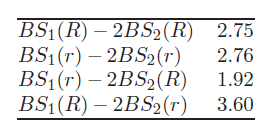
\includegraphics[scale=0.65]{spread_option_lower_upper_bound.png}
	\caption{linear combination of BScholes to get lower bound and upper bound }
\end{figure}

 \begin{center}
 	\includegraphics[scale=0.65]{Spread_option_Gobet1.png}
 \end{center}



 \begin{figure}[!htb]
 	\centering
 	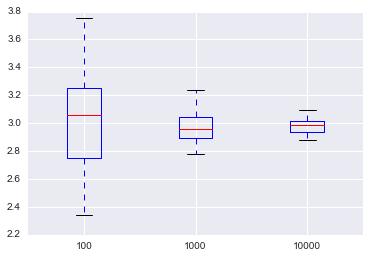
\includegraphics[scale=0.65]{BSDE_1D_different_rates_LSM_SPread_Option.png}
 	\caption{Simulation by LSM on polynomial basis (degree 5)}
	\end{figure}


\begin{figure}[!htb]
	\centering
	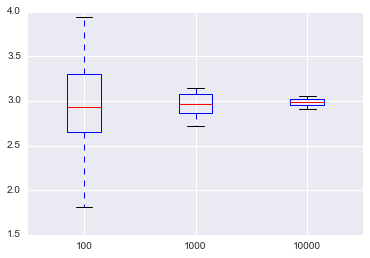
\includegraphics[scale=0.65]{BSDE_1D_different_rates_RF_SPread_Option.png}
	\caption{Simulation by Random Forest}
\end{figure}


\newpage

\subsection{Call Option}


\begin{itemize}
	\item $\xi(S_T)=(S_T-K)^+$
	\item parameters : 
	
	\begin{tabular}{c|c|c|c|c|c|c|c|c|c|c}
		$T$ & $m$* & $N$* & $S_0$  & $K$ & r& $\sigma$ & R & $\mu$ & n\_estimators & max\_leaf\_nodes\\
		\hline
		0.5  & 12 & 10 000 & 100  & 100 & $4\%$ & $20\% $ & $6\%$ & 0.06 & 100 & 100
	\end{tabular}
\end{itemize}

The seller of the option has always to borrow money to replicate the option in continuous time. Thus, $Y_0$ is given
by the Black–Scholes formula evaluated with interest rate $R$ :$Y_0 = 7.15$


\subsubsection{N increasing}



\begin{figure}[!htb]
	\centering
	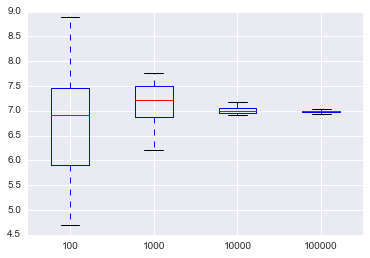
\includegraphics[scale=0.65]{2rates_LSM_N_increasing.png}
	\caption{Simulation by LSM on polynomial basis (degree 5)}
\end{figure}


\begin{figure}[!htb]
	\centering
	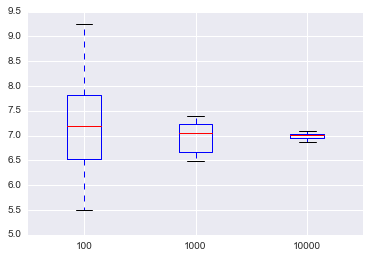
\includegraphics[scale=0.65]{2rates_Rforest_N_increasing.png}
	\caption{Simulation by Random Forest}
\end{figure}

\subsubsection{m increasing}
	
\end{document}	